\documentclass[tikz,border=8pt]{standalone}
\usepackage{amsmath}
\usetikzlibrary{arrows.meta,calc,decorations.pathmorphing}
\definecolor{ink}{HTML}{21352F}
\definecolor{teal}{HTML}{087F7B}
\definecolor{gold}{HTML}{C58B2A}
\definecolor{blue}{HTML}{4B77A8}
\definecolor{rose}{HTML}{B65A62}
\begin{document}
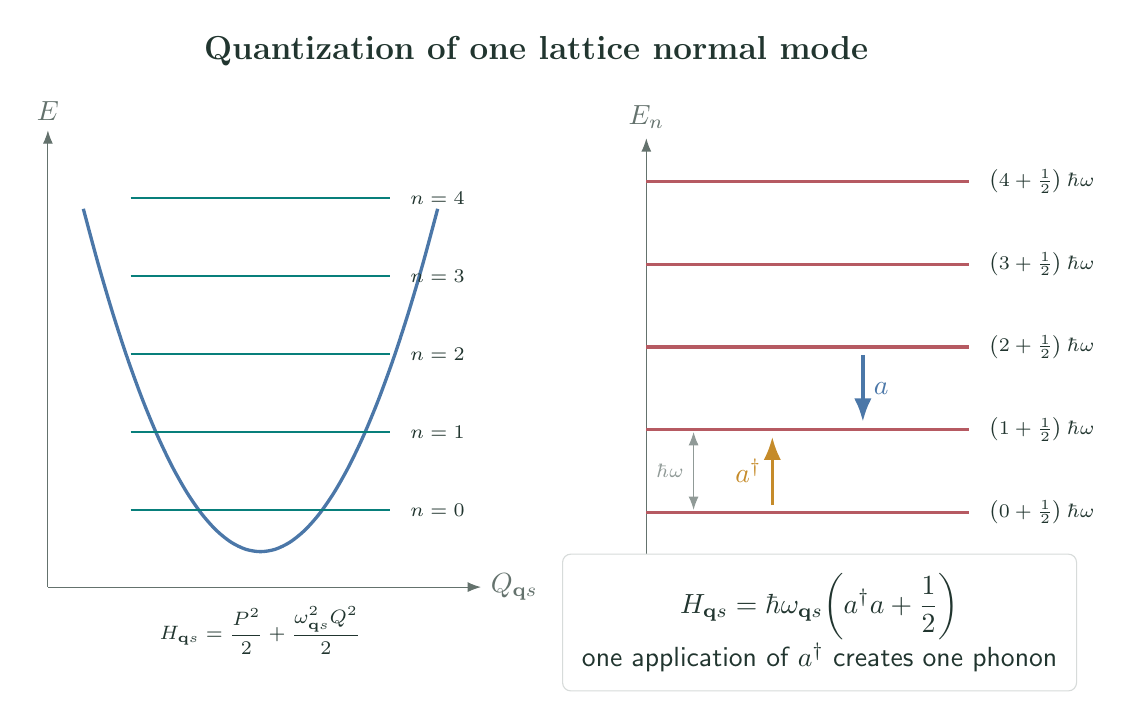
\begin{tikzpicture}[font=\sffamily,text=ink,>=Latex]
  \node[font=\bfseries\large] at (0,4.0) {Quantization of one lattice normal mode};
  \draw[->,ink!70] (-6.2,-2.8)--(-6.2,3.0) node[above] {$E$};
  \draw[->,ink!70] (-6.2,-2.8)--(-.7,-2.8) node[right] {$Q_{\mathbf q s}$};
  \draw[blue,very thick,domain=-2.25:2.25,smooth,variable=\x]
    plot ({-3.5+\x},{-2.35+0.86*\x*\x});
  \foreach \n/\y in {0/-1.82,1/-.83,2/.16,3/1.15,4/2.14}{
    \draw[teal,thick] (-5.15,\y)--(-1.85,\y);
    \node[font=\scriptsize,anchor=west] at (-1.72,\y) {$n=\n$};
  }
  \node[font=\scriptsize,align=center] at (-3.5,-3.35)
    {$\displaystyle H_{\mathbf q s}=\frac{P^2}{2}+\frac{\omega_{\mathbf q s}^2Q^2}{2}$};

  \draw[->,ink!70] (1.4,-2.45)--(1.4,2.9) node[above] {$E_n$};
  \foreach \n/\y in {0/-1.85,1/-.8,2/.25,3/1.3,4/2.35}{
    \draw[rose,very thick] (1.4,\y)--(5.5,\y);
    \node[font=\scriptsize,anchor=west] at (5.62,\y) {$\left(\n+\tfrac12\right)\hbar\omega$};
  }
  \draw[->,gold,very thick] (3.0,-1.76)--(3.0,-.89) node[midway,left] {$a^\dagger$};
  \draw[->,blue,very thick] (4.15,.15)--(4.15,-.70) node[midway,right] {$a$};
  \draw[<->,ink!50] (2.0,-1.82)--(2.0,-.83) node[midway,left,font=\scriptsize] {$\hbar\omega$};
  \node[draw=ink!18,rounded corners=3pt,fill=white,inner sep=7pt,align=center] at (3.6,-3.25)
    {$\displaystyle H_{\mathbf q s}=\hbar\omega_{\mathbf q s}\!\left(a^\dagger a+\frac12\right)$\\
     one application of $a^\dagger$ creates one phonon};
\end{tikzpicture}
\end{document}
